\documentclass[a4paper,12pt]{article}

\usepackage{my_pkg}
\usepackage{my_pkg2}

\title{Project 4: Adding Interaction [continuation of Projects 2 \& 3]}
\SetDocumentFooter{}{}

\begin{document}

\maketitle

\section{Objectives}

\myparagraph{In this assignment you will add interactive elements to your previous designs. Again, take care to use good software engineering practices. }

\section{Ground Rules}

\groundrules



\section{Assignment Instructions}

\begin{itemize}

\item Download the data set at \url{
http://www.calvin.edu/~stob/data/srsatact.csv}. This dataset contains standardized scores for all Calvin College 2004 seniors that have taken both the ACT and the SAT, together with their GPAs. There are 271 data points and 4 dimensions.

\item Modify your sketches from Project 2 and 3 to have a 800x600 resolution. 

\item To your BAR CHART, LINE CHART, and SCATTERPLOT, add an interaction that pops up data information when the mouse is over/clicks a particular bar/data point. Add to all of your plots the ability switch which attributes are being visualized.

\begin{center}
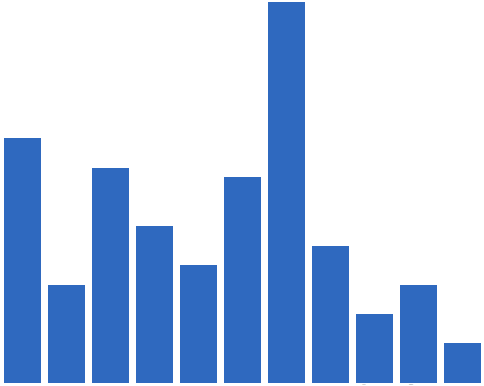
\includegraphics[width=4cm, height=2.5cm]{images/barchart.png} 
\hspace{15pt}
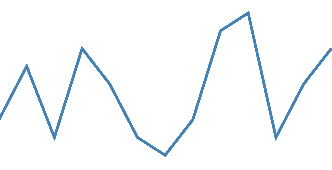
\includegraphics[height=2.5cm]{images/linechart.png} 
\hspace{15pt}
\fbox{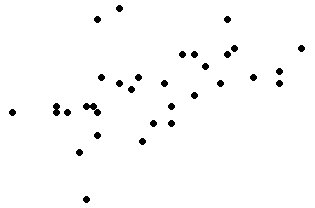
\includegraphics[height=2.5cm]{images/scatterplot.png}}
\end{center}

\item To your SCATTERPLOT MATRIX, add a detail view (an additional large scatterplot). Add an interaction such that when a plot is selected in the scatterplot matrix, it updates the detail view to those data attributes.

\begin{center}
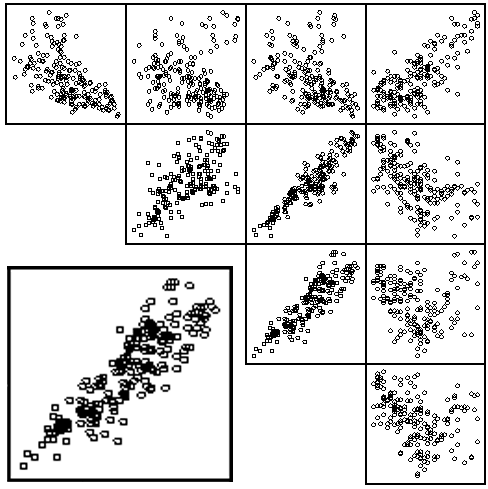
\includegraphics[width=4cm]{images/splom+detail.png} 
\end{center}

\item In addition, download (at least) TWO (2) of the other datasets provided on Canvas, and make sure they work with your sketches.

\item Add any additional interactions that you think will make your sketches more useful.

\item Modify your sketches such that they use additional visual channels to encode additional variables. Consider using color, size, shape, depth, etc. Your selection and their implementation will have an impact on your grade.

\item Add embellishments of your choice. These can include but are not limited to: axis lines, labels, and tick marks. Consider the margins for your embellishments (try to pick good values for the tick marks and a good number of them---not too many and not too few). Your selection and their implementation will have an impact on your grade.

\item Make your visualizations robust by designing them to support any data (number of elements or value range) and by designing them to support any size or aspect ratio of canvas.

\end{itemize}


\section{Submission}

\submission{project4}

\section{Grading and Feedback}

\feedback







\newpage


\begin{center}
{\huge Project 4 Peer Review}
\end{center}




\StartTable{Visual Design}

\AddMultipleChoiceElement{Visual Channels}
	{What visual channels were used to encode data? }
    { 
     \AddMCColumn{1.65cm}{\choice Position	\\ \choice Depth	\\ \choice Angle}
     \AddMCColumn{1.95cm}{\choice Curvature	\\ \choice Shape	\\ \choice Length}
     \AddMCColumn{2.3cm}{\choice Area		\\ \choice Volume  	\\ \choice Luminance/\\\ \ Saturation}
     \AddMCColumn{1.95cm}{\choice Color Hue	\\ \choice Texture	\\ \choice Motion/\\\ \ Animation}
    }
        
\AddElement{Intended/Unintended Encodings}
	{Do all of the visual encoding appear to be intended, or were some accidentally created?}
        {\choice Many\\Unintended}
        {\choice Few\\Unintended}
        {\choice All\\Intended} 
        
\AddElementExtended{Expressiveness of Encodings}
	{Are the visual encodings attached to the correct type of data for that 
    	encoding (i.e.\ are quantitative data attached to quantitative 
        encodings and categorical data to categorical encodings)?}
    {\choice Many\\Errors}
    {\choice Few\\Errors}
    {\choice Correctly\\Assigned} 
            
\AddElement{Effectiveness of Encodings}
	{Have the maximally effective visual encodings been selected in all cases? }
    {\choice Many\\Ineffective}
    {\choice Few\\Ineffective}
    {\choice Most\\Effective} 
        
\AddElement{Effective Use of Color}
	{Is color used in a same fashion? Do the colors chosen and the application 
    	of those colors make the visualization effective?}
    {\choice Mostly\\Ineffective}
    {\choice None\\Used}
    {\choice Highly\\Effective} 

\EndTable  

\vspace{15pt}

\StartTable{Design Considerations}

\AddElement{Clear, Detailed, and Thorough Labeling}
   	{Is appropriate and complete labeling used throughout or do 
      	missing labels require assumptions about the data?}
    {\choice No labels}
    {\choice Some Missing labels}
    {\choice Completely labeled} 
        
\AddElement{Missing Scales}
   	{Are scales provided for the data?}
	{\choice No Scales}
	{\choice Some Missing Scales}
	{\choice All Scales Present} 

\AddElement{Missing Legend}
	{Is a legend provided for the data? Does the legend provide useful 
    	information?}
	{\choice No Legend}
	{\choice Incomplete Legend}
	{\choice Complete Legend} 
        
        
\EndTable  


\StartTable{Design Considerations (cont.)}

\AddElement{Scale Distortion}
	{Is any scale distortion or deception used in the visualization?}	
	{\choice Severe Distortion}
	{\choice Minor Distortion}
	{\choice No Distortion} 
        
\AddElement{Lie Factor}
	{Is there any lie factor? How extreme is the lie factor?}
	{\choice Major Lie}
	{\choice Minor Lie}
	{\choice No Lie} 

\AddElement{Data/Ink Ratio}
	{Is the data to ink ratio reasonable? Could it be more efficient?}
	{Way Too $\square$~Little / $\square$~Much Ink}
	{Slightly Too $\square$~Little / $\square$~Much Ink}
	{\choice Perfect Amount of Ink} 
        
\AddElement{Chart Junk, Embellishments, Aesthetics}
	{Are appropriate embellishments used? Are the embellishments 
    	distracting? Do the embellishments add to the visualization?}
	{Way Too $\square$~Few / $\square$~Many Embellishments}
	{A Bit Too $\square$~Few / $\square$~Many Embellishments}
	{\choice Perfect Number of Embellishments} 
        
\AddElement{Data Density}
	{Has too much data been included in the visualization making 
    	interpretation difficult? } 
	{\choice Too Sparse}
	{\choice Expected}
	{\choice Too Dense} 
        
        
\AddElement{Gestalt Principals}
	{Have Gestalt principals been used to improve analysis?}
	{\choice No Gestalt Principals}
	{\choice Some Gestalt Principals}
	{\choice Many Gestalt Principals} 
        
\EndTable  
 
        
\vspace{15pt}   
 
\StartTable{Interaction Design}

\AddMultipleChoiceElement{Interaction Selection}
   	{What interaction mechanisms are being used?}
    {
     \AddMCColumn{2.45cm}{\choice Linked Views   \\ \choice Selection 	  \\ \choice Highlighting}
     \AddMCColumn{2.65cm}{\choice Filtering		 \\ \choice Aggregation	  \\ \choice Semantic Zoom}
     \AddMCColumn{2.70cm}{\choice Geometric Zoom \\ \choice Pan/Translate \\ \choice Rotate}
    }
        
\AddElementExtended{Interaction Effectiveness}
	{Are the interactions provided highly effective? In other words, does 
    	the visualization react in a manner that makes it easy to use or 
        capable of providing rich content?}
    {\choice Missing Key Interactions}
    {\choice Expected}
    {\choice Better Than Expected}
    
\EndTable



\newpage


\begin{center}
{\huge Project 4 Grading}
\end{center}

\begin{itemize}
	\item 4 Visualization - 2 points (0.5 points each)
	\item Required interactions - 5 points (1.25 points each)
	\item Additional interaction, embellishment, and additional Visual Channels - 1.5 points 
		\begin{itemize}
    		\item 0.5 points for none used
    		\item 1.0 point for a few
            \item 1.5 points for many
		\end{itemize}
	\item Code Professionalism - 1.5 points
		\begin{itemize}
            \item 0.75 no comments, no classes, "hard coded" values
            \item 1.0 minimally commented, few "hard coded" values
            \item 1.5 commented, used classes, few "hard coded" values
		\end{itemize}
\end{itemize}



\end{document}






\end{document}




